\documentclass{standalone}
\usepackage{tikz}
\usetikzlibrary{patterns, positioning}
\usepackage[sfdefault]{ClearSans} %% option 'sfdefault' activates Clear Sans as the default text font
\usepackage[T1]{fontenc}

\begin{document}
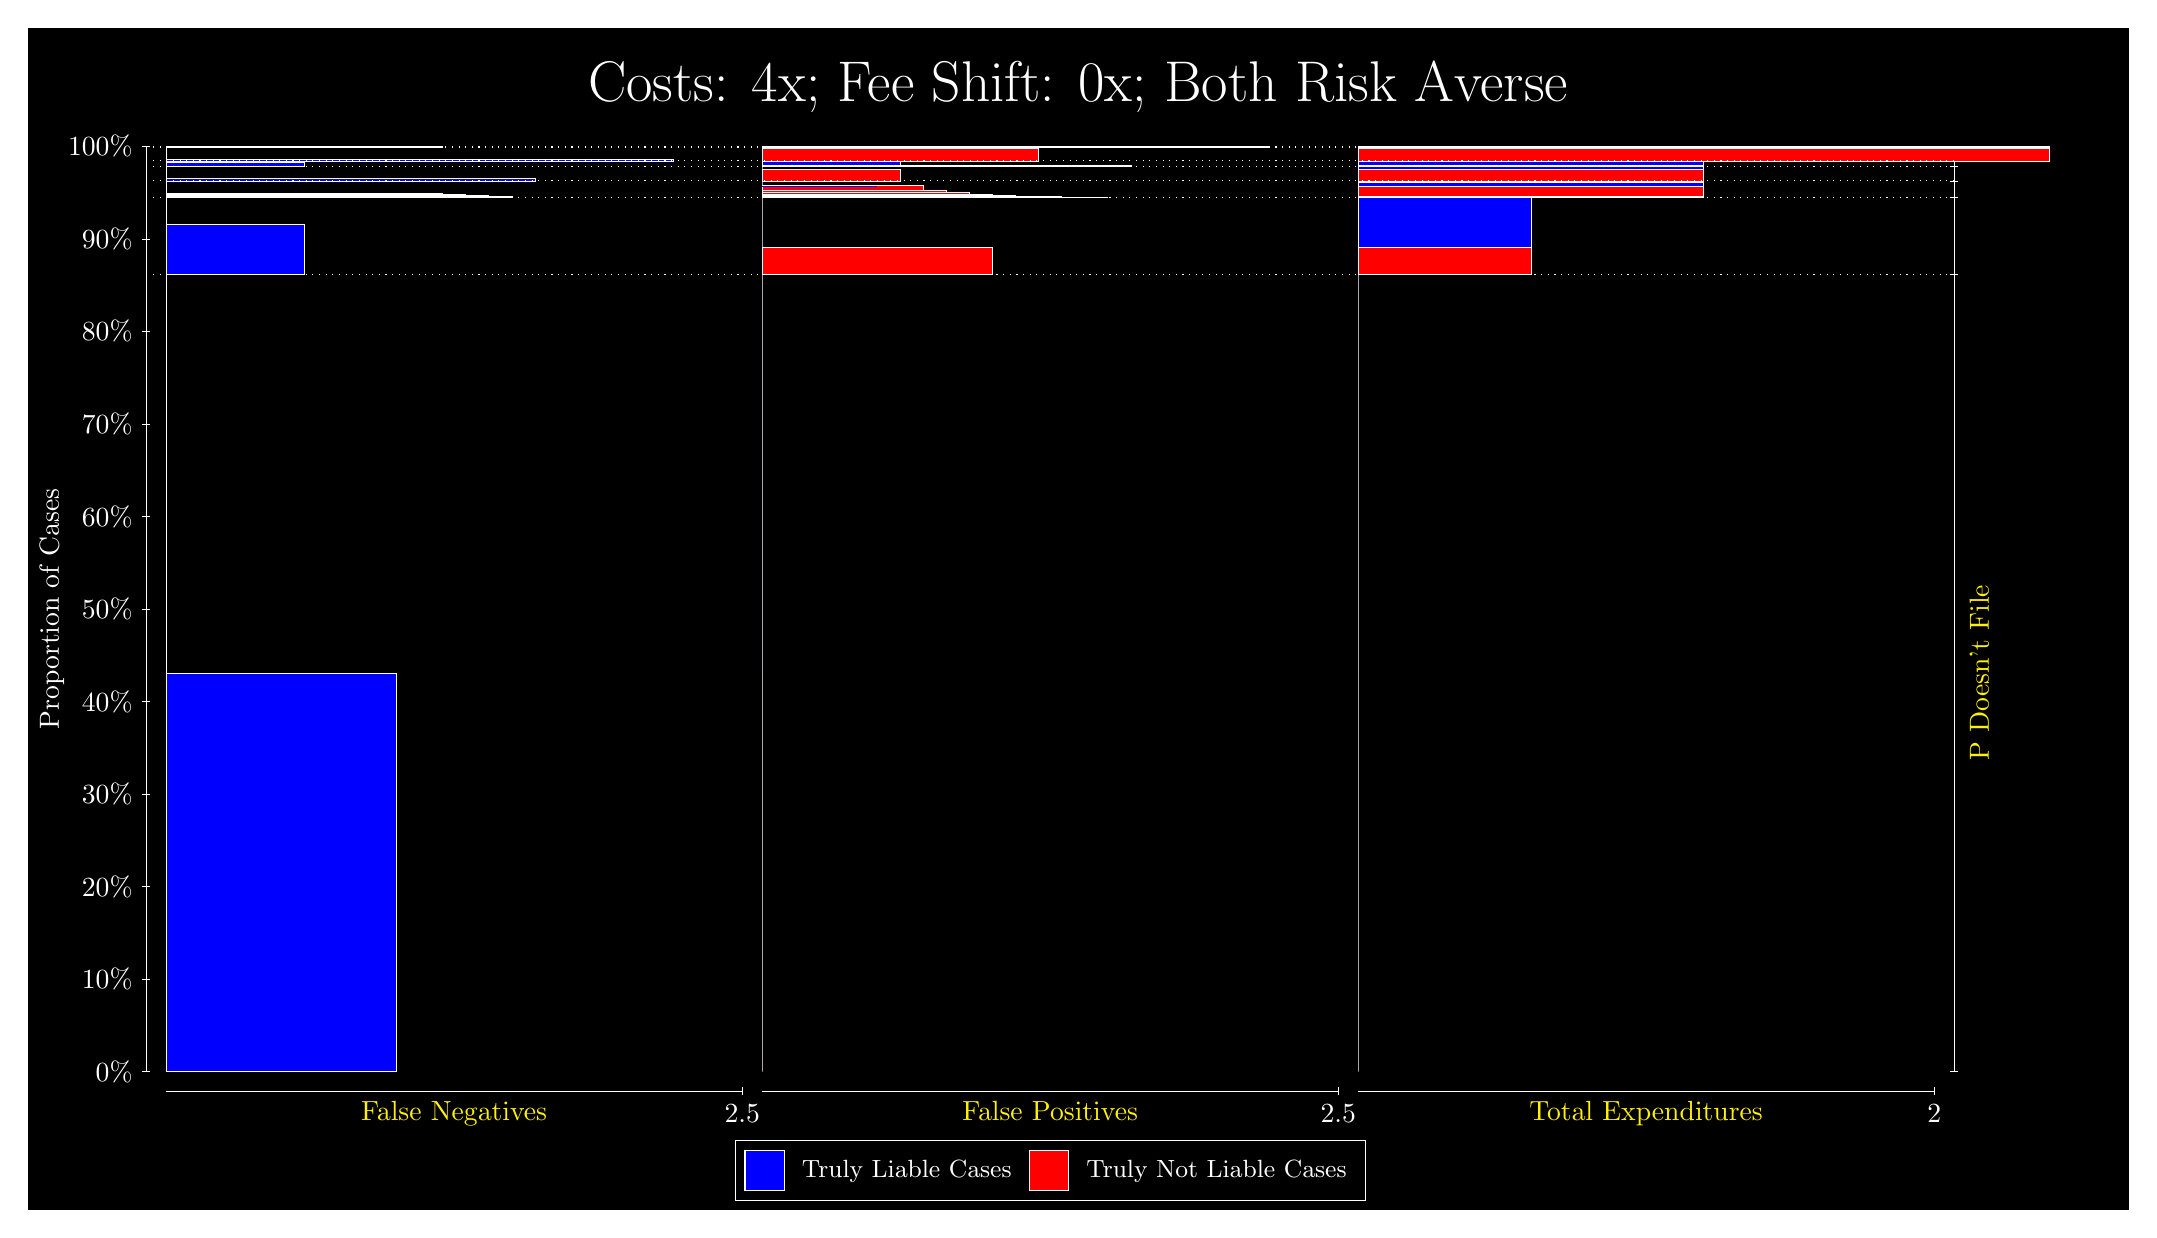
\begin{tikzpicture}
\draw[fill=black] (0,0) rectangle (26.667,15);
\draw[text=white] (0,13.5) rectangle (26.667,15) node[midway] {\huge Costs: 4x; Fee Shift: 0x; Both Risk Averse};
\draw[white, very thin] (1.5,1.75) -- (1.5,13.5);
\node[rotate=90, text=white, anchor=center] at (0.3, 7.625) {Proportion of Cases};
\draw[white, very thin] (1.45,1.75) -- (1.55,1.75);
\node[text=white, anchor=east] at (1.45, 1.75) {0\%};
\draw[white, very thin] (1.45,2.925) -- (1.55,2.925);
\node[text=white, anchor=east] at (1.45, 2.925) {10\%};
\draw[white, very thin] (1.45,4.1) -- (1.55,4.1);
\node[text=white, anchor=east] at (1.45, 4.1) {20\%};
\draw[white, very thin] (1.45,5.275) -- (1.55,5.275);
\node[text=white, anchor=east] at (1.45, 5.275) {30\%};
\draw[white, very thin] (1.45,6.45) -- (1.55,6.45);
\node[text=white, anchor=east] at (1.45, 6.45) {40\%};
\draw[white, very thin] (1.45,7.625) -- (1.55,7.625);
\node[text=white, anchor=east] at (1.45, 7.625) {50\%};
\draw[white, very thin] (1.45,8.8) -- (1.55,8.8);
\node[text=white, anchor=east] at (1.45, 8.8) {60\%};
\draw[white, very thin] (1.45,9.975) -- (1.55,9.975);
\node[text=white, anchor=east] at (1.45, 9.975) {70\%};
\draw[white, very thin] (1.45,11.15) -- (1.55,11.15);
\node[text=white, anchor=east] at (1.45, 11.15) {80\%};
\draw[white, very thin] (1.45,12.325) -- (1.55,12.325);
\node[text=white, anchor=east] at (1.45, 12.325) {90\%};
\draw[white, very thin] (1.45,13.5) -- (1.55,13.5);
\node[text=white, anchor=east] at (1.45, 13.5) {100\%};

\draw[white, very thin] (24.457,1.75) -- (24.457,13.5);
\draw[white, very thin] (24.407,1.75) -- (24.507,1.75);
\node[anchor=west] at (24.407, 1.75) {};
\draw[white, very thin] (24.407,11.876) -- (24.507,11.876);
\node[anchor=west] at (24.407, 11.876) {};
\draw[white, very thin] (24.407,12.847) -- (24.507,12.847);
\node[anchor=west] at (24.407, 12.847) {};
\draw[white, very thin] (24.407,13.061) -- (24.507,13.061);
\node[anchor=west] at (24.407, 13.061) {};
\draw[white, very thin] (24.407,13.246) -- (24.507,13.246);
\node[anchor=west] at (24.407, 13.246) {};
\draw[white, very thin] (24.407,13.315) -- (24.507,13.315);
\node[anchor=west] at (24.407, 13.315) {};
\draw[white, very thin] (24.407,13.491) -- (24.507,13.491);
\node[anchor=west] at (24.407, 13.491) {};
\draw[white, very thin] (24.407,13.5) -- (24.507,13.5);
\node[anchor=west] at (24.407, 13.5) {};

\draw[white, very thin, fill=blue] (1.75,1.75) rectangle (4.6775,6.8131);
\draw[white, very thin, fill=red] (1.75,6.8131) rectangle (1.75,11.876);
\draw[white, very thin, fill=blue] (1.75,11.876) rectangle (3.5065,12.511);
\draw[white, very thin, fill=red] (1.75,12.511) rectangle (1.75,12.847);
\draw[white, very thin, fill=blue] (1.75,12.847) rectangle (6.1413,12.86);
\draw[white, very thin, fill=blue] (1.75,12.86) rectangle (5.8486,12.877);
\draw[white, very thin, fill=blue] (1.75,12.877) rectangle (5.5558,12.896);
\draw[white, very thin, fill=blue] (1.75,12.896) rectangle (5.2631,12.898);
\draw[white, very thin, fill=blue] (1.75,12.898) rectangle (4.9703,12.902);
\draw[white, very thin, fill=blue] (1.75,12.902) rectangle (4.6775,12.905);
\draw[white, very thin, fill=blue] (1.75,12.905) rectangle (4.3848,12.907);
\draw[white, very thin, fill=blue] (1.75,12.907) rectangle (4.092,12.909);
\draw[white, very thin, fill=blue] (1.75,12.909) rectangle (3.7993,12.91);
\draw[white, very thin, fill=red] (1.75,12.91) rectangle (1.75,13.061);
\draw[white, very thin, fill=blue] (1.75,13.061) rectangle (6.4341,13.096);
\draw[white, very thin, fill=red] (1.75,13.096) rectangle (1.75,13.246);
\draw[white, very thin, fill=blue] (1.75,13.246) rectangle (3.5065,13.303);
\draw[white, very thin, fill=red] (1.75,13.303) rectangle (1.75,13.315);
\draw[white, very thin, fill=blue] (1.75,13.315) rectangle (8.1906,13.333);
\draw[white, very thin, fill=red] (1.75,13.333) rectangle (1.75,13.491);
\draw[white, very thin, fill=blue] (1.75,13.491) rectangle (5.2631,13.496);
\draw[white, very thin, fill=red] (1.75,13.496) rectangle (1.75,13.5);
\draw[white, very thin, fill=red] (9.3189,1.75) rectangle (9.3189,6.8131);
\draw[white, very thin, fill=blue] (9.3189,6.8131) rectangle (9.3189,11.876);
\draw[white, very thin, fill=red] (9.3189,11.876) rectangle (12.246,12.212);
\draw[white, very thin, fill=blue] (9.3189,12.212) rectangle (9.3189,12.847);
\draw[white, very thin, fill=red] (9.3189,12.847) rectangle (13.71,12.851);
\draw[white, very thin, fill=red] (9.3189,12.851) rectangle (13.417,12.854);
\draw[white, very thin, fill=red] (9.3189,12.854) rectangle (13.125,12.861);
\draw[white, very thin, fill=red] (9.3189,12.861) rectangle (12.832,12.869);
\draw[white, very thin, fill=red] (9.3189,12.869) rectangle (12.539,12.879);
\draw[white, very thin, fill=red] (9.3189,12.879) rectangle (12.246,12.886);
\draw[white, very thin, fill=red] (9.3189,12.886) rectangle (11.954,12.92);
\draw[white, very thin, fill=red] (9.3189,12.92) rectangle (11.661,12.946);
\draw[white, very thin, fill=red] (9.3189,12.946) rectangle (11.368,12.999);
\draw[white, very thin, fill=blue] (9.3189,12.999) rectangle (10.783,13);
\draw[white, very thin, fill=blue] (9.3189,13) rectangle (10.49,13.001);
\draw[white, very thin, fill=blue] (9.3189,13.001) rectangle (10.197,13.004);
\draw[white, very thin, fill=blue] (9.3189,13.004) rectangle (9.9044,13.007);
\draw[white, very thin, fill=blue] (9.3189,13.007) rectangle (9.6116,13.01);
\draw[white, very thin, fill=blue] (9.3189,13.01) rectangle (9.3189,13.061);
\draw[white, very thin, fill=red] (9.3189,13.061) rectangle (11.075,13.211);
\draw[white, very thin, fill=blue] (9.3189,13.211) rectangle (9.3189,13.246);
\draw[white, very thin, fill=red] (9.3189,13.246) rectangle (14.003,13.258);
\draw[white, very thin, fill=blue] (9.3189,13.258) rectangle (11.075,13.315);
\draw[white, very thin, fill=red] (9.3189,13.315) rectangle (12.832,13.474);
\draw[white, very thin, fill=blue] (9.3189,13.474) rectangle (9.9044,13.491);
\draw[white, very thin, fill=red] (9.3189,13.491) rectangle (15.759,13.495);
\draw[white, very thin, fill=blue] (9.3189,13.495) rectangle (12.832,13.5);
\draw[white, very thin, fill=red] (16.888,1.75) rectangle (16.888,6.8131);
\draw[white, very thin, fill=blue] (16.888,6.8131) rectangle (16.888,11.876);
\draw[white, very thin, fill=red] (16.888,11.876) rectangle (19.083,12.212);
\draw[white, very thin, fill=blue] (16.888,12.212) rectangle (19.083,12.847);
\draw[white, very thin, fill=red] (16.888,12.847) rectangle (21.279,12.858);
\draw[white, very thin, fill=blue] (16.888,12.858) rectangle (21.279,12.862);
\draw[white, very thin, fill=red] (16.888,12.862) rectangle (21.279,12.992);
\draw[white, very thin, fill=blue] (16.888,12.992) rectangle (21.279,13.046);
\draw[white, very thin, fill=red] (16.888,13.046) rectangle (21.279,13.057);
\draw[white, very thin, fill=blue] (16.888,13.057) rectangle (21.279,13.061);
\draw[white, very thin, fill=red] (16.888,13.061) rectangle (21.279,13.211);
\draw[white, very thin, fill=blue] (16.888,13.211) rectangle (21.279,13.246);
\draw[white, very thin, fill=red] (16.888,13.246) rectangle (21.279,13.258);
\draw[white, very thin, fill=blue] (16.888,13.258) rectangle (21.279,13.315);
\draw[white, very thin, fill=red] (16.888,13.315) rectangle (25.67,13.474);
\draw[white, very thin, fill=blue] (16.888,13.474) rectangle (25.67,13.491);
\draw[white, very thin, fill=red] (16.888,13.491) rectangle (25.67,13.495);
\draw[white, very thin, fill=blue] (16.888,13.495) rectangle (25.67,13.5);
\draw[white, dotted] (1.5,11.876) -- (24.457,11.876);
\draw[white, dotted] (1.5,12.847) -- (24.457,12.847);
\draw[white, dotted] (1.5,13.061) -- (24.457,13.061);
\draw[white, dotted] (1.5,13.246) -- (24.457,13.246);
\draw[white, dotted] (1.5,13.315) -- (24.457,13.315);
\draw[white, dotted] (1.5,13.491) -- (24.457,13.491);
\draw[white, very thin] (1.75,1.5) -- (9.0689,1.5);
\node[text=yellow, anchor=north] at (5.4094, 1.5) {False Negatives};
\draw[white, very thin] (9.0689,1.45) -- (9.0689,1.55);
\node[text=white, anchor=north] at (9.0689, 1.45) {2.5};

\draw[white, very thin] (9.3189,1.5) -- (16.638,1.5);
\node[text=yellow, anchor=north] at (12.978, 1.5) {False Positives};
\draw[white, very thin] (16.638,1.45) -- (16.638,1.55);
\node[text=white, anchor=north] at (16.638, 1.45) {2.5};

\draw[white, very thin] (16.888,1.5) -- (24.207,1.5);
\node[text=yellow, anchor=north] at (20.547, 1.5) {Total Expenditures};
\draw[white, very thin] (24.207,1.45) -- (24.207,1.55);
\node[text=white, anchor=north] at (24.207, 1.45) {2};

\node[text=yellow, centered, rotate=90] at (24.777, 6.8131) {P Doesn't File};







\draw (12.978300999999998,1.5) node[draw=none] (baseCoordinate) {};
\begin{scope}[align=center]
        \matrix[scale=0.5, draw=white, below=0.5cm of baseCoordinate, nodes={draw}, column sep=0.1cm]{
            \node[rectangle, draw, minimum width=0.5cm, minimum height=0.5cm, fill=blue] {}; &
            \node[draw=none, font=\small, text=white] (B) {Truly Liable Cases}; &
            \node[rectangle, draw, minimum width=0.5cm, minimum height=0.5cm, fill=red] {}; &
            \node[draw=none, font=\small, text=white] (B) {Truly Not Liable Cases}; \\
            };
\end{scope}

\end{tikzpicture}
\end{document}